% !TEX root = main.tex




\subsection{Comparison to existing PV technologies}

Comparison of the ASF to other PV technologies and the UCTE electricity mix is highlighted in Figure \ref{fig:compPV}. We can see in this figure that the ASF without shading benefits is inferior to all other technologies. It is only with the added shading benefits that we really see the advantages of the adaptive system. \textcolor{magenta}{\textit{(I think we need to provide and explain the e+ simulation results somehwere.)}}
We can also see that the utilisation of the ASF in an area where the electricity mix has low GWP intensity such as Switzerland also has disadvantages. It is capable of out performing Silicone based technologies but is still inferior to simply mounted CIGS panels. Note that even the panels themselves of the ASF, without the BOS, is still lower that the CIGS installation. This is due to the added inefficiencies as the panels are not always at the optimum position to the sun.


\begin{figure}[H]
\begin{center}
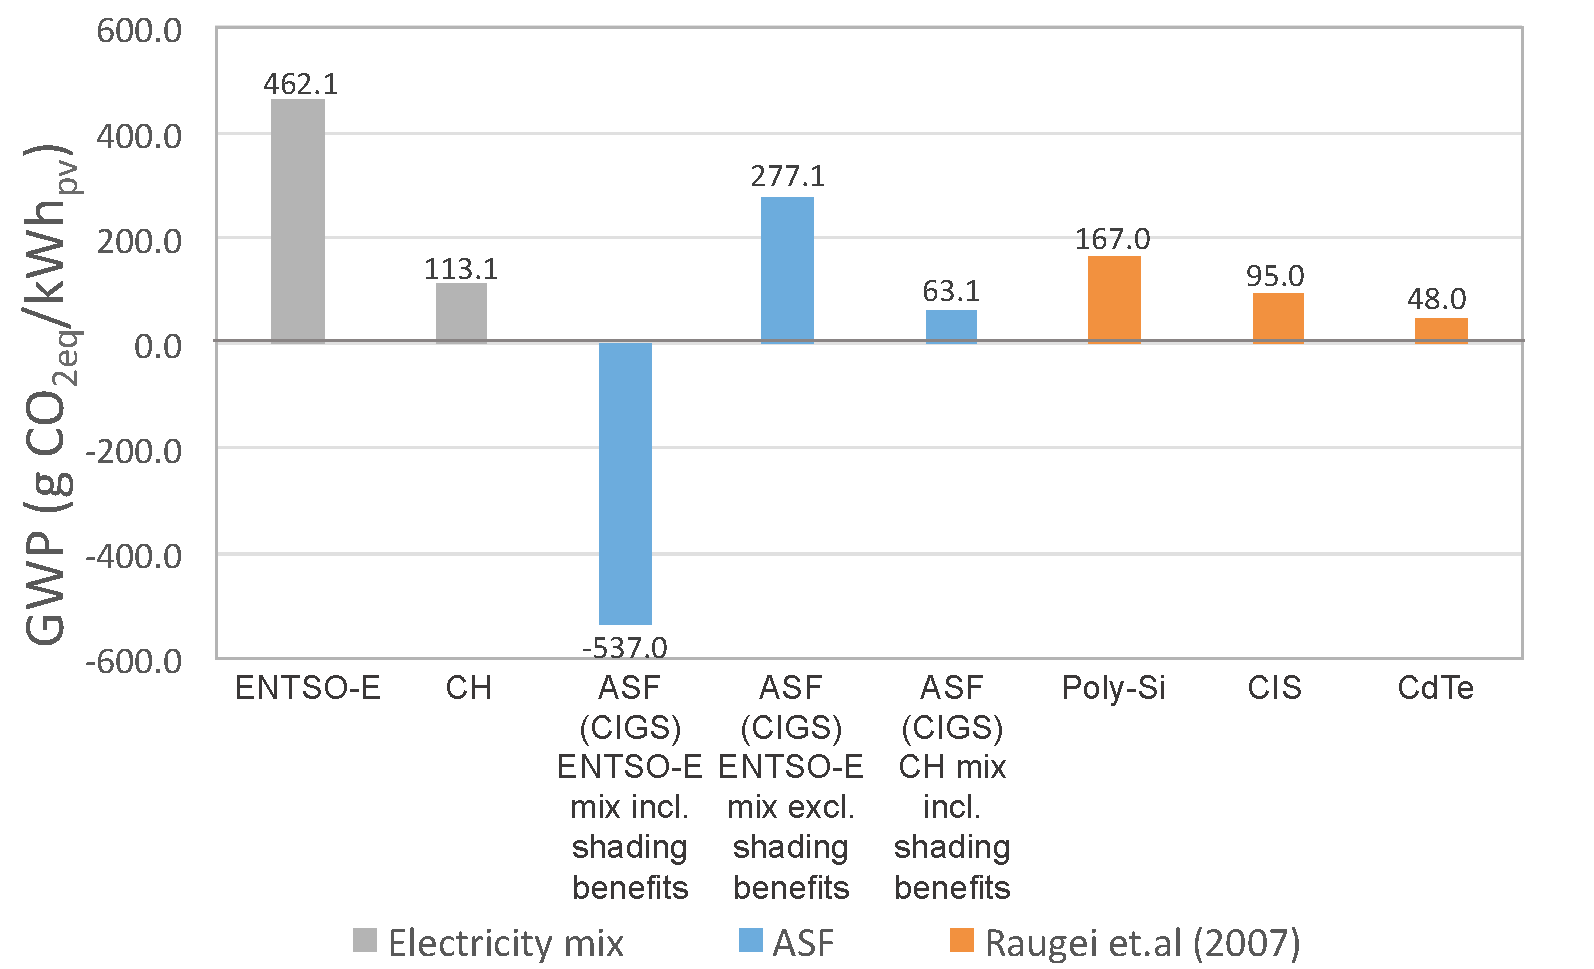
\includegraphics[width=10cm, trim= 0cm 0cm 0cm 0cm,clip]{compPV.pdf}
\caption{Comparison of thin-film and BOS to other PV technologies. I would add some extra columns, one without shading, one with the ASF in Switzerland, one with the ASF in Europe}
\label{fig:compPV}
\end{center}
\end{figure}




